%% HEADER
%%%%%%%%%%%%%%%%%%%%%%%%%%%%%%%%%%%%%%%%%%%%%%%%%%%%%%%%%%%%%
%%
%%
\newcommand{\hyperrefpdfauthor}{}
\newcommand{\hyperrefpdftitle}{}
\newcommand{\hyperrefpdfsubject}{}
\newcommand{\hyperrefpdfkeywords}{}
\newcommand{\hyperrefpdfborder}{0}
\documentclass{styles/wissdoc-kw-eng}

\usepackage{pdfpages}
\usepackage[printonlyused]{acronym}

% % newer acronym packaged dont use bflabel anymore,
\providecommand\aclabelfont{} % the new command ist aclabelfont however, we also need to be backwards compatible so... we do it like this
\renewcommand{\aclabelfont}[1]{\normalfont{\normalsize{#1}}\hfill} % keine serifenlose schrift für acronym

% newer acronym packaged dont use bflabel anymore, to not fail the statement below provide the command if not existing
\providecommand\bflabel{}
\renewcommand{\bflabel}[1]{\aclabelfont{#1}}

%\usepackage{acronym}
\usepackage{subfigure}

\usepackage{float}
\floatstyle{ruled}
\newfloat{listing}{htbp}{lop}[chapter]
\floatname{listing}{Listing}

\usepackage[hang,center,nooneline]{caption}
\captionsetup[figure]{font={small,sf}}
\captionsetup[table]{font={small,sf}}
\captionsetup[listing]{font={small,sf}}
\usepackage[absolute]{textpos}
\usepackage{styles/etoolbox}


%% Normales LaTeX oder pdfLaTeX? %%%%%%%%%%%%%%%%%%%%%%%%%%%%
%% ==> Das neue if-Kommando "\ifpdf" wird an einigen wenigen
%% ==> Stellen benötigt, um die Kompatibilität zwischen
%% ==> LaTeX und pdfLaTeX herzustellen.
%\newif\ifpdf
%\ifx\pdfoutput\undefined
%    \pdffalse              %%normales LaTeX wird ausgeführt
%\else
%    \pdfoutput=1
%    \pdftrue               %%pdfLaTeX wird ausgeführt
%\fi


%% Fonts für pdfLaTeX %%%%%%%%%%%%%%%%%%%%%%%%%%%%%%%%%%%%%%%
%% ==> Nur notwendig, falls keine cm-super-Fonts installiert
\ifpdf
	\usepackage{ae}       %%Benutzen Sie nur eines dieser Pakete:
	%\usepackage{zefonts}  %%je nachdem, welches Sie besitzen.
\else
	%%Normales LaTeX - keine speziellen Fontpackages notwendig
\fi


%% Deutsche Anpassungen %%%%%%%%%%%%%%%%%%%%%%%%%%%%%%%%%%%%%
%\usepackage[T1]{fontenc}
%\usepackage[utf8]{inputenc}

%% zur Zitaten des Quelltextes%%%%%%%%%%%%%%%%%%%%%%%%%%%%%%%
% "final" forces printing of all listings, even if the global "draft" is set
\usepackage[final]{listings}
\lstset{
    basicstyle=\footnotesize\ttfamily,
    tabsize=4,
    numberstyle=\tiny\color{gray},
    numbersep=5pt,
    numbers=left,
    captionpos=b,
    abovecaptionskip=0pt,
    belowcaptionskip=0pt,
    aboveskip=10pt,
    belowskip=0pt,
    floatplacement=tbp,
    frame=topline,
    framerule=.1pt,
    framesep = 3pt,
    }
\renewcommand\lstlistingname{\textbf{Listing}}
% This is only kept for backwards compatibility. You should never have to use it. Use the listing-environment instead.
%\DeclareCaptionFormat*{lstruled}{{\bfseries#1\small\space\normalfont#3\hrule height.1pt depth0pt}\par}
%\captionsetup[lstlisting]{format=lstruled,singlelinecheck=false}

%% mehrere Abbildungen in eine %%%%%%%%%%%%%%%%%%%%%%%%%%%%%%
\usepackage{subfigure}

%% Packages für Formeln %%%%%%%%%%%%%%%%%%%%%%%%%%%%%%%%%%%%%
\usepackage{amsmath}
\usepackage{amsthm}
\usepackage{amsfonts}

%% Zeilenabstand %%%%%%%%%%%%%%%%%%%%%%%%%%%%%%%%%%%%%%%%%%%%
\usepackage{setspace}
%\singlespacing        %% 1-zeilig (Standard)
%\onehalfspacing       %% 1,5-zeilig
%\doublespacing        %% 2-zeilig


%% Andere Packages %%%%%%%%%%%%%%%%%%%%%%%%%%%%%%%%%%%%%%%%%%
%\usepackage{a4wide} %%Kleinere Seitenränder = mehr Text pro Zeile.
\usepackage{fancyhdr} %%Fancy Kopf- und Fußzeilen
%\usepackage{longtable} %%Für Tabellen, die eine Seite überschreiten
\usepackage{lscape}
\usepackage{rotating}
%\usepackage[htt]{hyphenat} %Trennung von Typewriter-Schriften
%\usepackage{listings}
\usepackage{pstricks-add}
\usepackage{tikz}
\usepackage{pgfplots}


% Tabellen mit Center und left
\usepackage{tabularx,colortbl} % colored table background
\newcolumntype{C}[1]{>{\centering\arraybackslash}p{#1}}
\newcolumntype{R}[1]{>{\raggedleft\arraybackslash}p{#1}}
% Table spacings
\newcommand\T{\rule{0pt}{2.5ex}\rule[-1.0ex]{0pt}{0pt}}
\newcommand\B{\rule[-1.0ex]{0pt}{0pt}}

\definecolor{slightgray}{gray}{.90}


%% Definitionen %%%%%%%%%%%%%%%%%%%%%%%%%%%%

% Command to provide a figure caption that also specifies a .settings file.
\newcommand*{\captionsettings}[2]{%
  \caption[{#1}]{%
    #1%
    \\\hspace{\linewidth}%
    \textcolor{gray}{\texttt{.settings} file: \texttt{#2}}%
  }%
}


%% zur Benutzung bei ergänzenden Daten%%%%%%%%%%%%%%%%%%%%%%%%
%\usepackage{endnotes}
%\renewcommand{\notesname}{Konfigurationsdaten der Messreihen}
%\renewcommand{\theendnote}{\Alph{endnote}}
%\renewcommand{\enotesize}{\normalsize}

%\hyphenation{Sensor-netz-werk
%}

%%%%%%%%%%%%%%%%%%%%%%%%%%%%%%%%%%%%%%%%%%%%%%%%%%%%%%%%%%%%%
%% DOKUMENT
%%%%%%%%%%%%%%%%%%%%%%%%%%%%%%%%%%%%%%%%%%%%%%%%%%%%%%%%%%%%%
\begin{document}

%% Dateiendungen für Grafiken %%%%%%%%%%%%%%%%%%%%%%%%%%%%%%%
%% ==> Sie können hiermit die Dateiendung einer Grafik weglassen.
%% ==> Aus "\includegraphics{titel.eps}" wird "\includegraphics{titel}".
%% ==> Wenn Sie nunmehr 2 inhaltsgleiche Grafiken "titel.eps" und
%% ==> "titel.pdf" erstellen, wird jeweils nur die Grafik eingebunden,
%% ==> die von ihrem Compiler verarbeitet werden kann.
%% ==> pdfLaTeX benutzt "titel.pdf". LaTeX benutzt "titel.eps".
%\ifpdf
%    \DeclareGraphicsExtensions{.pdf,.jpg,.png}
%\else
%    \DeclareGraphicsExtensions{.eps}
%\fi

\pagestyle{empty} %%Keine Kopf-/Fusszeilen auf den ersten Seiten.

\ifnotdraft{
%% Deckblatt %%%%%%%%%%%%%%%%%%%%%%%%%%%%%%%%%%%%%%%%%%%%%%%%
\frontmatter
% !TEX root =  ../thesis.tex

\titlehead{
%	\hfill
%	
\includegraphics[width=10cm,keepaspectratio]{logos/rwth_comsys_bild_cmyk}
} % end titlehead


\begin{titlepage}

\begin{textblock*}{10cm} (12.7cm,2.7cm)

\includegraphics[width=10cm,keepaspectratio]{logos/rwth_comsys_bild_cmyk}
\end{textblock*}

\let\footnotesize\small \let\footnoterule\relax

\hbox{}
\vfill

\centering

\begin{doublespace} 
{ \huge\sffamily\textbf{Your Awesome Thesis Title \\ \vspace{-0.7em}
(Which May Also Be Quite Long \\ \vspace{0.2em}
And Stretch Several Lines) Here}}
\end{doublespace}
\vskip 2cm

{\large\sffamily

BachelorMasterDiploma Thesis\\[5pt]
\textbf{Your Name Here}
\vskip 1cm

This work was submitted to the\\[5pt]
\textbf{Chair of Communication and Distributed Systems\\[5pt]
        RWTH Aachen University, Germany}
\vskip 2cm

Adviser(s):
\vskip 2mm
Dipl.-Inform. Erika Mustermann\\
Max Mustermann, M.$\,$Sc.
\vskip 5mm
Examiners:
\vskip 2mm
Prof.~Dr.-Ing. Klaus Wehrle\\
Prof.~Dr. Second Albert Einstein
\vskip 1cm

\begin{tabular}{R{6cm}p{6cm}}
Registration date:  & 2016-??-?? \\
Submission date:    & 2017-??-?? \\
\end{tabular}

} %\large\sffamily

\vfill

\end{titlepage}

\cleardoublepage
% !TEX root =  ../thesis.tex
\includepdf[pages={1},offset=75 -75,pagecommand={
\begin{tikzpicture}[remember picture,overlay,shift={(current page.center)}]
\coordinate (de_begin-de_generic) at (5.4,10.3);
\coordinate (de_end-de_generic) at (6.4,10.3);
\coordinate (de_begin-de_bachelor) at (6.5,10.3);
\coordinate (de_end-de_bachelor) at (9,10.3);
\coordinate (de_begin-de_master) at (-5.35,9.8);
\coordinate (de_end-de_master) at (-3.2,9.8);
\coordinate (en_begin-en_generic) at (3.2,9.35);
\coordinate (en_end-en_generic) at (3.9,9.35);
\coordinate (en_begin-en_bachelor) at (4.0,9.35);
\coordinate (en_end-en_bachelor) at (5.9,9.35);
\coordinate (en_begin-en_master) at (6.0,9.35);
\coordinate (en_end-en_master) at (7.65,9.35);
\node at (-5.5,12.1)
       [text width=7cm,rounded corners,below right]
{
\textcolor{red}{Lehmann, Marc}
};
\node at (3.25,12.1)
       [text width=5cm,rounded corners,below right]
{
\textcolor{red}{} % This is optional
};
% ===== for type generic uncomment the next 4 lines =====
% \draw[line width=1mm] (de_begin-de_bachelor) -- (de_end-de_bachelor);
% \draw[line width=1mm] (de_begin-de_master) -- (de_end-de_master);
% \draw[line width=0.5mm] (en_begin-en_bachelor) -- (en_end-en_bachelor);
% \draw[line width=0.5mm] (en_begin-en_master) -- (en_end-en_master);
% ===== for type de_bachelor uncomment the next 4 lines =====
%\draw[line width=1mm] (de_begin-de_generic) -- (de_end-de_generic);
%\draw[line width=1mm] (de_begin-de_master) -- (de_end-de_master);
%\draw[line width=0.5mm] (en_begin-en_generic) -- (en_end-en_generic);
%\draw[line width=0.5mm] (en_begin-en_master) -- (en_end-en_master);
% ===== for type de_master uncomment the next 4 lines =====
 \draw[line width=1mm] (de_begin-de_generic) -- (de_end-de_generic);
 \draw[line width=1mm] (de_begin-de_bachelor) -- (de_end-de_bachelor);
 \draw[line width=0.5mm] (en_begin-en_generic) -- (en_end-en_generic);
 \draw[line width=0.5mm] (en_begin-en_bachelor) -- (en_end-en_bachelor);
%
\node at (-5.5,8.95)
       [text width=16.5cm,rounded corners,below right]
{
\textcolor{red}{
Incentivizing Peers to Contribute in a Low-Latency Name-Lookup-system}
};
\node at (-5.5,2.35)
       [text width=7cm,rounded corners,below right]
{
Aachen, \textcolor{red}{15.07.2019}
};
\node at (-5.5,-8.7)
       [text width=7cm,rounded corners,below right]
{
Aachen, \textcolor{red}{15.07.2019}
};
\end{tikzpicture}
}]{Formular_Eidesstattliche_Versicherung_neu.pdf}

\cleardoublepage
\cleardoublepage

\begin{center}
\paragraph{Abstract}
\hrulefill
\end{center}
TODO

\cleardoublepage
\cleardoublepage

\chapter*{Acknowledgments}
TODO

\cleardoublepage

% Titelseite hatte noch normale Tabellen. Von hier ab sollen alle
% Tabellen laut style-Vorgaben sans serif sein.
\AtBeginEnvironment{tabular}{\sffamily}
\AtBeginEnvironment{tabularx}{\sffamily}

%% Inhaltsverzeichnis %%%%%%%%%%%%%%%%%%%%%%%%%%%%%%%%%%%%%%%
\tableofcontents %Inhaltsverzeichnis
\cleardoublepage %Das erste Kapitel soll auf einer ungeraden Seite beginnen.
} % end ifnotdraft

\pagestyle{fancy} %%Ab hier die Kopf-/Fusszeilen: headings / fancy / ...

%%%%%%%%%%%%%%%%%%%%%%%%%%%%%%%%%%%%%%%%%%%%%%%%%%%%%%%%%%%%%
% einzelne Kapitel
%%%%%%%%%%%%%%%%%%%%%%%%%%%%%%%%%%%%%%%%%%%%%%%%%%%%%%%%%%%%%
%\input{commands}

\mainmatter
\chapter{Introduction}
- TODO update submission date?
- TODO spellcheck

This thesis proposes a system built on top of a distributed hash table (DHT)
forcing its users to become nodes contributing to it. It does so by punishing
those who don't with a bad quality of service. The motivation is to use the DHT
for a name-lookup service and give its users many nodes to query for privacy
reasons.

\section{Privacy in Name-Lookup}
The domain name system (DNS) is a service essential for the Internet, its
primary purpose being the mapping of domain names to IP addresses. In general, a
name mapping service that allows looking up the network address associated with
a name belonging to some entity (e.g. a server, or a user identity) is
indispensable for any large network. Using the network addresses themselves is
impractical because they are often not permanently assigned.

The way name resolution is typically handled for private end users is that they
send all their lookups to one DNS server that they were made aware of by their
internet service provider. When they communicate with another host for the first
time, e.g. to access a web site or send an email, they send a DNS request to
that server. The response is then likely cached for a while by their
operating system or their browser, but the DNS server still gets at least an
initial request and knows which host they are likely communicating with. Thus,
DNS requests are privacy-sensitive data that allow the server to build user
profiles.

This issue, the accumulation of sensitive name resolution queries at central
locations, is the motivation behind this thesis. Note that just encrypting
traffic with DNS servers doesn't help, the issue isn't eavesdroppers on the
connection, it's all of a user's DNS meta data heaping up at one central server.
The operator of the DNS server doesn't even have to have malicious intentions,
or in fact any intentions to use the data. Simply the fact that data from many
users accumulates there makes the server a worthwhile target for infiltration by
malicious agents.

The chosen approach to address the issue is to spread out name-lookup requests
to many servers rather than using just one resolver. This doesn't make
incursions on users' privacy impossible, but should significantly increase the
work needed to gather a relevant amount of data, especially when attempted on a
large scale targeting many users at once. The thinking is that a foreign party
having access to a little bit of privacy-sensitive data is relatively benign,
that they are only able to build a meaningful profile once they have acquired a
considerable volume. With many lookup servers available, users are able to
choose themselves how far they want to spread out their requests.

\section{Goal}
There needs to be a great number of servers for this to work. This thesis
introduces a system in which these servers are the nodes of a \ac{DHT}, and the
mapping from name to network address the \emph{records} stored in it. The main
purpose of this system is to ensure that there is a great number of nodes. To
achieve this, its main focus lies on incentivizing every user of the lookup
service to not just use it, but to become a \emph{peer}, i.e. a node of the
\ac{DHT} that also contributes resources to providing it.

A good motivating use case, and one that's useful to keep in mind, is a
peer-to-peer chat system. Every peer has a fixed \emph{ID} by which he is known
to the others, but the network addresses can change frequently. The \ac{DHT} is
used to store the mapping from ID to network address. In fact, the rest of the
thesis assumes that each peer stores exactly one record containing his
\emph{reachability information} in the \ac{DHT}, where the key is equal to his
own peer ID (the key of a record is also referred to as the ID of the record).

Since network addresses change, peers frequently need to look up the current
addresses of others they want to chat with. Sending all these lookups to one
central server would give that server a pretty good picture of what a peer is
doing. Spreading them throughout the \ac{DHT} means a lot of people know a
little, but no single party knows enough to be useful.

Accessing a record is somewhat latency sensitive. While it is not a real-time
application, it becomes annoying if the lookup before sending a message takes
too long. Furthermore, it must be possible to update records, and for these
updates to be disseminated throughout the \ac{DHT} quickly. But we can assume
that the records are fairly small, containing just an ID, an address, and maybe
some additional information.

The system is likely capable of supporting other applications than such a chat
system, notably ones with fewer of the limiting assumptions. But for the sake of
simplicity, and to focus on the more interesting aspects, they are kept in place
here.

Another underlying assumption is that the users are selfish. They want to expend
as little storage space, CPU time and network bandwidth as possible. Without any
addition to the \ac{DHT}, they can do that whether or not they contribute
themselves; one more node is not going to make a big difference in the grand
scheme, and certainly not provide them a benefit. Using the DHT but not
contributing is called free-riding. The fact that peers want to use the service
and enjoy the benefit of having many peers to choose from to do their lookups is
the leverage the system exploits: peers who aren't contributing are given a
worse quality of service.

Whitewashing is a similar exploit in which peers use the system until the level
of service they are given is not satisfactory anymore, then leave and join again
with a new identity. The system addresses this by being suspicious of newcomers,
giving them a low quality of service that only improves once they have proven
themselves trustworthy.

\section{Necessity of Incentives}
The assumption that all peers are entirely selfish and need to be made to see a
benefit to themselves for every action required of them is very pessimistic. It
begs the question whether such a system is even necessary. Storing a few small
records containing reachability information and responding to queries concerning
them only takes little resources. Given that, it's not unreasonable to be
optimistic and believe that people wishing to use such a service are willing to
contribute to it.

In fact, McGee and Sk{\aa}geby\cite{mcgee2004gifting} survey the motivation of
users of a peer-to-peer file sharing service to \emph{gift}, i.e. to seed
without reward. They find that there are users motivated by ideology
("information wants to be free"), as well as ones acting altruistically, i.e.
for whom the act of sharing files itself is the motivation.

A later paper\cite{ripeanu2006gifting} related to this examines motivations for
gifting in BitTorrent. The authors find that social characteristics strongly
influence sharing behavior, a user base that has a culture of sharing outside
the file sharing application will gift more in file sharing. They also find that
a small subset of the most active uploaders is responsible for a majority of the
uploads (in 95\% of torrents, over half the file is uploaded by the top 10\% of
uploaders).

This suggests that, while gifting, or generous behavior, in peer-to-peer
applications exists, relying on it may not be suitable for the system proposed
in this thesis. It could be suggested to peers that participating in offering
the service makes it better, in hopes of inviting generous peers' contributions,
as proposed in a blog post of the Tor Project\cite{dingledine2009incentive_tor}.
The problem is that this may mostly just encourage the small subset of the most
generous peers. But the system absolutely needs many peers participating so
users can spread out their queries. Few peers doing most of the work is actually
counterproductive to the privacy goal.

One could also argue that it should be sufficient to write an implementation of
the \ac{DHT} in which peers contribute by default, perhaps with no option of
disabling it. The overhead of this is small, so users wouldn't change the
software for a small benefit. Ripeanu et al.\cite{ripeanu2006gifting} even
recognize the difficulty of configuring a BitTorrent client to free-ride as a
contribution to the low levels of free-riding. But then a problem will arise if
an alternative implementation leaves out the contribution, e.g. out of laziness
or for security reasons (less code means less space for vulnerabilities).

While there is no certainty that incentives are absolutely necessary, there are
some indications that they are. Cox et al.\cite{cox2002serving}, who explore the
possibility of serving DNS via peer-to-peer also state "We need to find models
in which people have incentives to run servers rather than just take free rides
on others’ servers.". In the end, it may be best just to be prepared for the
worst.

Whitewashing is a peer leaving and then rejoining the system with a different ID
in order to shed previous bad reputation. This attack is viable only in systems
where new users are given some trust upon joining, which they can subsequently
lose. In the system proposed here, peers joining a query group start at the very
bottom, namely 0 reputation (and reputation is non-negative). Rejoining thus
doesn't afford them any benefit.

\section{Outline}
- TODO check this for accuracy
- TODO explain the structure of the thesis, explain *why* it is structured in
  such a way, why the chapter are arranged in this order (and how they build on
  each other)

Chapter~\ref{chap:related_work} TODO

Chapter~\ref{chap:background} gives brief introductions into techniques and
concepts that are the basis of the work presented in this thesis.

Chapter~\ref{chap:system_description} describes the incentive system in detail.

Chapter~\ref{chap:implementation} describes the implementation of a simplified
implementation of the system, and a simulation used to evaluate it.

Chapter~\ref{chap:rep_avail} presents an evaluation of the system with regard to
the ability of cooperative peers to quickly establish themselves in the system
and enjoy use of the service without hindrance.

Chapter~\ref{chap:performance} examines the performance achievable by the system
theoretically and compares it with alternatives.

Chapter~\ref{chap:future_work} TODO

Chapter~\ref{chap:conclusion} concludes and gives an outlook towards interesting
open problems concerning the system.

\chapter{Background}
\label{chap:background}
\section{Distributed Hash Tables}
Distributed hash tables (DHTs) are a method of distributing data storage to
nodes in a network. From an abstract point of view, they are just hash tables
that map keys to values. They are appealing because they offer robust data
storage without the need for a central authority.

The keys usually have fixed length, the values, or records, can be arbitrary
data. Some care should be taken to ensure there are no collisions in keys. Using
a cryptographic hash of the record itself is a possibility achieving that.

Each node in the DHT stores a number of the records. In the language of this
thesis, it is \emph{responsible for} them. The key of a record determines who is
responsible for it, and there is a distance metric measuring how far a node is
to being responsible for a record. In the DHT used in this thesis every node has
an ID that has the same format as the keys in the DHT. Nodes are responsible for
those records the keys of which have the same prefix as their ID.

A node in the network needs not know all other nodes, but for any key it must
know another node closer to that node. Then it is possible to route to any
record stored in the DHT. The node can ask the closer node for the record, which
in turn asks another node closer, eventually reaching a responsible node.

Records can be created, updated and deleted by contacting the node responsible
for the corresponding key.

A useful robustness feature is replication, in which more than one node is
responsible for each record. This way, if a node fails, the record is not lost.
All the nodes responsible for the same records must stay in contact to
synchronize their records, making each other aware of new and updated records as
well as deletions.

Load balancing is another advanced feature that's useful if some records are
much more popular, or much bigger than others. To achieve it, the mapping from
node to the records the node is responsible for must be mutable. More nodes are
then made responsible for the records that generate a lot of traffic.

- TODO explain routing in p-grid/kademlia style dht (picture with the tree)

\section{Discrete Event Simulation}
A discrete event simulation framework simulates a system by processing events at
discrete times. This can be implemented deterministically, making the
simulations reproducible.

In execution, the framework maintains the current
\emph{simulated time}, i.e. the time within the simulation, which counts up as
the simulation progresses. The central part of the framework is the event queue,
which contains events, each together with the time at which it should be
triggered.

An event is the unit of action in the framework and models something taking
place. This can for example be a message being sent over the network. Events can
be \emph{triggered}, meaning the action they represent is executed. They can
then mutate the state of the system, as well as place new events on the event
queue. For example, the message-sent event could modify the sender's state for
outbound messages and place a message-received event in the event queue a little
bit in the future.

The simulation is initialized by placing at least one event in the queue. When
it is started, the framework continually pops the next event (the one with the
lowest trigger time) from the event queue, forwards the simulated time to the
event's trigger time, and triggers the event.

If the last event taken from the queue doesn't place any new events, the
simulation ends. But there are also other useful termination criteria, like
reaching a (wall clock) time limit, reaching a simulated time limit, or e.g.
reaching a certain number of events processed.

The procedure described is serial, i.e. single-threaded. Discrete event
simulations can be parallelized, but this takes some effort. Race conditions can
occur if two successive events are removed from the event queue and triggered
concurrently. These must be detected, the system rolled back, and the events
processed again sequentially. This issue can be made less likely by distributing
events across threads such that events that are likely to cause race conditions
are processed in the same thread.

In this thesis, the SimPy framework~\cite{simpy} was used. It is written in
Python, allowing for quick iteration of the model. However, it can't be
parallelized, so the simulation is strictly single-threaded. Parallelizing was
considered difficult considering that the point of the system is that everyone
is able to spread out messages to a lot of other users. Thus, there would likely
not be clusters that could be assigned to one thread.

\section{Game Theory}
TODO
- trembles, cite that paper
- collusion/sybil
- free riding, whitewashing
\subsection{Reputation Management}
- credit-debit, credit-only

\chapter{System Description}
\label{chap:system_description}
\section{Assumptions and Prerequisites}
The system described in this chapter assumes that, for any pair of peers, there
is a reliable way for them to communicate at all times. In practice, this means
that each peer is able to establish and maintain a TCP connection with any other
peer. Messages may be delayed e.g. due to congestion, but must arrive
eventually. Issues arising from e.g. NAT that would make it impossible to
contact a peer directly, but also complete link failures that cause connections
to time out are considered out of scope.

While network delays can be dealt with, jitter should be low enough that future
delays can be predicted from past ones with reasonable accuracy.

Peers are assumed to have clocks, all of which are synchronized. Minor
variations are tolerable, though (typical accuracy of NTP is definitely enough).

Access to the DHT is assumed to be equally distributed. This includes firstly
that the records are equally popular, i.e. each of them has the same likelihood
of being queried for. Secondly, all peers send the same volume of queries.
Sections~\ref{sec:desc_load_balancing}
and~\ref{sec:desc_credit_only_vs_credit_debit} discuss the consequences of these
assumptions not holding.

\subsection{Types of Peers}
\subsubsection{Selfish}
Selfish peers are the central type of peer this thesis focuses on, and the one
discussions are about unless otherwise indicated. They are lazy and only willing
to expend resources (network bandwidth, CPU time, memory) for their own benefit.
They only want to use them in order to be very likely in a position to receive
service quickly at all times. There is no explicit valuation determining what
"very likely" means to a peer. Rather, the reputation buffer described in
Section~\ref{sec:impl_coop_defect_behavior} acts as a proxy for it, determining
the reliably a peer receives good service.

When they don't see a benefit for themselves in taking a particular action they
won't do it, even if the protocol requires them to. Finding incentives for this
type of peer is a central part of this thesis, and achieved by threatening to
lower the quality of service. Section~\ref{sec:desc_rationale} goes into more
detail on the motivation of selfish peers.

\subsubsection{Generous}
\label{sec:desc_generous_peers}
Generous peers are in a way the opposite of selfish peers. They don't care about
their own benefit and strive to make others' lives easier, or at least they
behave in such a way. This can actually become a problem, since it reduces the
incentive for other peers to do work, thus counteracting the goal of providing
many peers to interact with. The system has to take measures against this kind
of behavior. Section~\ref{sec:desc_rep_system} goes into more detail.

Generous peers may actually be malicious, trying to attract a lot of traffic in
order to build profiles. This is briefly discussed in
Section~\ref{sec:desc_attacks_generous}, but otherwise out of the scope of this
thesis.

\subsubsection{Contented}
\label{sec:desc_contented_peers}
Contented peers don't care about the quality of service they receive and thus
can't be incentivized via it. These could e.g. be running on slow devices
without direct user interaction. If they appear in large numbers, they may cause
problems. Section~\ref{sec:rep_avail_selection_rep_sorted_contented} discusses
one such problem, but other than that, this type of peers is considered out of
scope.

\subsubsection{Colluding/Sybils}
Colluding peers are multiple selfish peers working together in order to do less
work while enjoying the same level of service. Sybils (peers performing a Sybil
attack) are single peers acting under multiple identities trying to achieve the
same thing.

These are out of scope of the implementation, but some ideas are presented in
Section~\ref{sec:desc_collusion_sybil_attacks} on how they may be dealt with.


\subsubsection{Malicious}
Malicious peers are motivated by causing harm to others or by disrupting the
entire system. They are willing to invest resources towards that goal without
the need for further incentives. One possible motivation is vengeance, peers
seeking to cause harm to particular peers who have wronged them. These are also
beyond the scope of this thesis.

\section{Organization}
\subsection{Overview}
The underlying DHT for the system is one in the style of Kademlia or P-Grid,
briefly described in Section~\ref{sec:background_dhts}. Every peer has a unique
\emph{ID} that he chooses himself, and every \emph{record} in the DHT has a
unique ID of the same length. In fact, each peer may store exactly one record
under its own ID, containing reachability information. As mentioned previously,
this constraint was added for simplicity. Under these circumstances, querying
for a record stored in the DHT is done in order to learn how to contact a peer.
For this reason, the phrase "querying for a peer (with some ID)" is frequently
used in this thesis to mean querying for a record in the DHT with that peer's
ID.

These IDs are bit strings of fixed length and routing takes place along a binary
tree formed by them. It may be possible to adapt the system to work with DHT
using a different routing scheme, such as Chord. See
Section~\ref{sec:desc_querying} for details on how querying is handled in the
DHT used by the system.

Every peer stores a number of records of the DHT, he is \emph{responsible} for
these records. A number of other peers is also responsible for these same
records, and the peer stays in contact with them in a \emph{sync group}. In
these groups, peers synchronize their information about stored records, like the
creation of a new one, or the update of an existing one. See
Section~\ref{sec:desc_sync_groups} for details on sync groups.

The system implements a reputation system in which peers have a
\emph{reputation} that is tracked within \emph{query groups}. A peer has a
separate non-negative, real-valued reputation value in each such group that he
is a member of. This value is initialized to 0 upon entering the group. The
other members of these groups are the peer's \emph{query peers}, and every one
of them knows the current reputation of each of the other query peers. They are
the ones to whom the peer forwards queries he can't answer himself directly. The
way query groups are created, how they are managed, and what dynamics arise from
this is not examined in this thesis, but there proposals and more details on
query groups in Section~\ref{sec:desc_query_groups}.

A peer receives a \emph{reward}, i.e. an increase of his reputation in a query
group if he performs a \emph{cooperative action} towards a peer in that group.
Conversely, he receives a \emph{penalty}, i.e. a decrease of his reputation in a
query group, if he performs a \emph{defecting action} towards a peer in that
group. However, reputation is non-negative, and so penalties have no effect if
the peer has 0 reputation. The terms \emph{cooperative} and \emph{defecting} are
chosen following the terms from game theory. An example (in fact the only
example relevant for the implementation considered in this thesis) of a
cooperative action is responding to a query with the correct answer within the
time frame demanded by the system's \emph{rules} (the set of parameters).
Examples of a defecting action are not responding to a query, responding with an
answer that states that the query could not be resolved, or responding too early
or too late. See Section~\ref{sec:desc_rep_management} for details on how
reputation is tracked in query groups.

The reputation peers earn is used to determine the quality of service they
receive. Peers responding to queries are mandated to apply a \emph{penalty
delay} (not to be confused with a \emph{penalty}, described above) appropriate
to the reputation of the querying peer. This includes deliberately delaying the
answer. The rules of the system define a \emph{penalty threshold reputation} (or
just \emph{penalty threshold}), which is the amount of reputation a peer must be
at or above in order to be entitled to receive responses without penalty delay
from query peers in the corresponding query group. If the querying peer's
reputation is below the penalty threshold, the penalty delay in seconds is
chosen inversely proportional to the peer's reputation: the more reputation, the
lower the delay.

Reputation is credit-only, i.e. once a peer has passed the penalty threshold he
may send as many queries as he likes and is entitled to delay-free service, he
doesn't have to "pay" with having his reputation reduced for a query.

Above the penalty threshold, \emph{reputation attenuation} makes it more
difficult for peers to gain further reputation. A distinction is made between
\emph{raw reputation} and \emph{effective reputation}. The latter is calculated
from the former by attenuating it. See Section~\ref{sec:attenuation} for the
rationale behind this and a more detailed description.

During operation, pairs of peers exchange messages without other peers knowing
their content or even being aware communication is taking place at all.
Disagreements may occur between peers about whether the other's behavior was
within the rules of the system. For example, a querying peer may claim that the
responding peer took too long to respond and should receive a penalty, while the
responding peer insists he responded in time and should receive a reward.
Neither of the peers is able to prove his claim. A distributed \emph{complaint
system} needs to be in place that can make rulings in these situations. Such a
system is not part of the implementation in this thesis, and there may be very
complex dynamics arising from such a system that are not foreseeable without a
simulation. However, a proposal is presented in
Section~\ref{sec:desc_complaints}.

At many points, the system relies on messages being authenticated. It is assumed
that all messages exchanged between peers are signed to prevent one peer
impersonating another. Since peers only store one record in the DHT with their
own ID as key, these records are also signed. Peer IDs are chosen to be
fingerprints of the peer's public key, so that there doesn't have to be a
mapping from peer ID to public key. The full public key can be distributed once
a peer learns about another peer for the first time, e.g. as supplementary
information in the peer's record in the DHT.

\subsection{Sync Groups}
\label{sec:desc_sync_groups}
Every peer has a \emph{routing prefix}, which is a prefix of the peer's ID. The
length of the routing prefix is fixed in the rules of the system and the same
for all peers. A peer is responsible for all records whose ID starts with his
routing prefix. In short, he is responsible for the routing prefix. He maintains
contact with other peers who have the same routing prefix; these peers make up
his sync group and are called his \emph{sync peers}.

Sync peers keep each other apprised of changes to their record\footnote{As a
reminder, in this simplified version, peers store exactly one record in the DHT,
where the key is their own ID.}. When it needs to be updated, they broadcast the
new record to all their sync peers, who then update their local copy.

Since every peer stores exactly one record in the DHT under his own ID, creating
a new record to be maintained in the sync group is equivalent to joining the
group. To do this, the peer needs to know at least one other peer who is already
a member of the sync group and gives him the contact information of all other
sync peers. Then he broadcasts his new record to all the members.

Conversely, deleting a record is equivalent to leaving the group. In this case,
the peer simply broadcasts a notification to his sync peers.

Sync groups are relevant to replication within the DHT. Every peer's record is
replicated as many times as there are peers in the sync group. The mean
replication factor in the DHT is $\frac{n}{2^l}$, where $n$ is the total number
of peers participating in the DHT, and $l$ is the length of the routing prefix
in bits.

No fixed replication factor can be guaranteed in this way, since the routing
prefixes are determined by the peer IDs, which peers choose themselves. It may
happen that one routing prefix is chosen by many fewer peers than another,
giving their records much lower replication. To address this, load balancing is
possible, see Section~\ref{sec:desc_load_balancing}.

\subsection{Querying}
\label{sec:desc_querying}
If a peer wants to get hold of a record (the key of which is called the
\emph{target ID}), he must send a query to another peer, the recipient. He
queries a peer known to him who is \emph{closer to} the target ID. This is the
case if the overlap of the recipient's routing prefix with the target ID is
greater than the overlap of the peer's own routing prefix with the target ID.
The overlap $o(a, b)$ of a bit string $a_i, i \in \{1, \ldots, n\}$ of length
$n$ and a bit string $b_j, j \in \{1, \ldots, m\}$ of length $m$ is defined as
\[o(a, b) = \max_{k \in \{0, \ldots, \min(n, m)\}} a_i = b_i \forall i \in \{1,
\ldots, k\}.\]

Note that, in case the peer's routing prefix overlaps entirely with the target
ID, i.e. it is also a prefix of the target ID, the peer himself is responsible
for the record and should know it and not need to query anyone.

In case the recipient doesn't know the record himself, further querying is
necessary. There are multiple possibilities for handling this. The simplest of
them is a recursive query, analogous to recursive DNS queries, in which the
recipient of the initial query does all the work. He selects a peer closer to
the target ID and sends him a query. This peer again may need to query another
peer. But this can only be the case a finite number of times, since the next
peer queried must always be closer to the target ID, so eventually one is
reached who is responsible for it. Once a response arrives at one of the peers
in this chain of queries, it is used to respond to the peer who queried him.
There are alternatives to this procedure discussed in
Section~\ref{sec:desc_recursive_vs_iterative}.

In this chain of queries, one of them may fail or time out. The peer should then
retry the query with a different suitable peer. If he has exhausted all the
possibilities, the query has failed. If the peer was querying on behalf of
another, he should send a \emph{fail response}, indicating he is unable to
resolve the query.

Peers may elect to send multiple queries at once instead of waiting for one to
fail first. This reduces the risk of letting the querying peer wait
unnecessarily, especially if a timeout has to be waited out.

There may not exist a record under the target ID. In that case, the recipient of
the query should respond with a message that indicates this. A peer who isn't
responsible for the routing prefix of the target ID isn't guaranteed to be aware
of changes to its records though. For example, a new one may recently have been
added. Only peers in the sync group responsible for that routing prefix are
synchronizing information about relevant records. The sync group therefore is an
\emph{authority} for the routing prefix, and so are its sync peers. Therefore,
the responding peer must include a signature from an authoritative sync peer in
the message that indicates no record exists for the target ID.

Instead of querying for a complete ID, the target ID can be a prefix of an ID of
arbitrary length (it can even be empty). A correct response to such a query is
any record whose ID starts with the target ID. This is useful for learning about
peers to complete one's subprefix coverage (see
Section~\ref{sec:desc_query_groups}). A response stating that no record with the
target ID exists in this context means that no record exists in the entire DHT
whose ID starts with the target ID.

Additionally, when querying for a prefix, a querying peer may specify a number
of IDs or prefixes of IDs to exclude. The response must not match any of the
excluded IDs or prefixes. This is useful for peers looking for peers with
certain prefixes: They can list the IDs of peers they already know in order to
learn about peers they don't yet. If they then receive a response stating that
no record with the target ID exists, it means that they already know all peers
matching the target ID.

\subsection{Query Groups}
\label{sec:desc_query_groups}
Query groups are the second kind of group employed by the system. Every peer may
be in multiple query groups, other members are called his \emph{query peers}.
Query peers are the pool of potential recipients of queries.

Query groups are the unit within which reputation is tracked. Reputation is
synchronized within a query group, so that every peer is aware of each of his
query peer's reputations. In order for this to remain scalable, query groups
should be kept reasonably small. Section~\ref{sec:desc_rep_management} contains
details on how the reputation record is kept up to date.

\subsubsection{Rewards, Penalties, and Penalty Delays}
The reason peers should only send queries to query peers is that their
reputation determines the quality of service they're entitled to receive. When
receiving a query, peers are required to consider the reputation of the querying
peer and apply a penalty delay, if applicable, i.e. to purposefully delay the
response. Failing to do so is itself a defecting action and incurs a penalty.
The appropriate penalty delay is $\max(0, t - r)$, where $t$ is the penalty
threshold reputation and $r$ is the peer's reputation.

The penalty thresholg is part of the rules of the system, and thus known to
everyone, and $r$ is known to all query peers. This means the sender of the
query knows what penalty delay is appropriate for his query. If a response has
not arrived $d + l$ after the query has been sent, where $l$ is another
parameter to account for network latency, the response is late and the querying
peer must apply a penalty for a timeout. If the response arrives after less than
$d$ time has passed, the response is early and the querying peer must apply a
penalty for an early query.

Otherwise, the response has arrived within the correct time frame. In that case,
the querying peer must either apply a penalty for a failed response if the
response indicates that the recipient is unable to answer the query, or apply a
reward for a successful query if the response appears to contain the correct
information.

Furthermore, the querying peer may, through one or more additional queries, find
that the response was incorrect. This can be either because it was outdated, or
because it falsely claimed that no record existed for the target ID, when in
fact it did. In that case, the querying peer must apply a penalty for an
incorrect response.\footnote{To detect whether a record is outdated, they
contain a timestamp giving the last time they were changed. There should be some
leeway given, though. No penalty should be applied if the record has only just
been updated.}

\subsubsection{Subprefix Coverage}
Section~\ref{sec:desc_querying} described the process of sending a query and
stated that a peer wishing to send a query must send it to a recipient who is
closer to the target ID of the query. This requires the peer to know such a
recipient for every possible target ID. This is the case if the peer has
complete \emph{subprefix coverage}.

A bit string is a peer's \emph{subprefix} iff it is no longer than the peer's
routing prefix, all of it but the final bit is a prefix of the peer's routing
prefix, but the whole thing is not.

Formally, a bit string $s_i, i \in \{1, \ldots, n\}$ of length $n$ is a
subprefix of a peer with routing prefix $p_j, j \in \{1, \ldots, m\}$ of length
$m$ iff $n \leq m \land s_i = p_i, i \in \{1, \ldots, n - 1\} \land s_n \neq
p_n$. In other words, $s$ is a subprefix of $p$ iff $s$ is no longer than $p$
and the bitwise XOR of $s$ and an appropriately truncated $p$ takes the form
$00\ldots001$. Each peer therefore has $m$ different subprefixes, one each of
every length in $\{1, \ldots, m\}$. Figure~\ref{fig:subprefixes} illustrates
subprefixes on an example.

A peer has complete subprefix coverage iff for each of his subprefixes he knows
at least one query peer for whose ID that subprefix is a prefix. No matter what
target ID he wishes to query for, he always knows a query peer closer to it: He
simply selects the query peer corresponding to the subprefix that has the
largest overlap with the target ID. That peer is at least one bit closer, namely
the last bit of the subprefix that is different for the peer sending the query.

Moreover, there is a 50\% chance that the query peer's routing prefix overlaps
by at least 2 bits (in general, a $\frac{1}{n}$ chance it overlaps by at least
$n$ bits), just by luck. This means steps in the routing can be "skipped", an
authoritative peer for the target ID is reached sooner.

\begin{figure}[t]
  \centering
  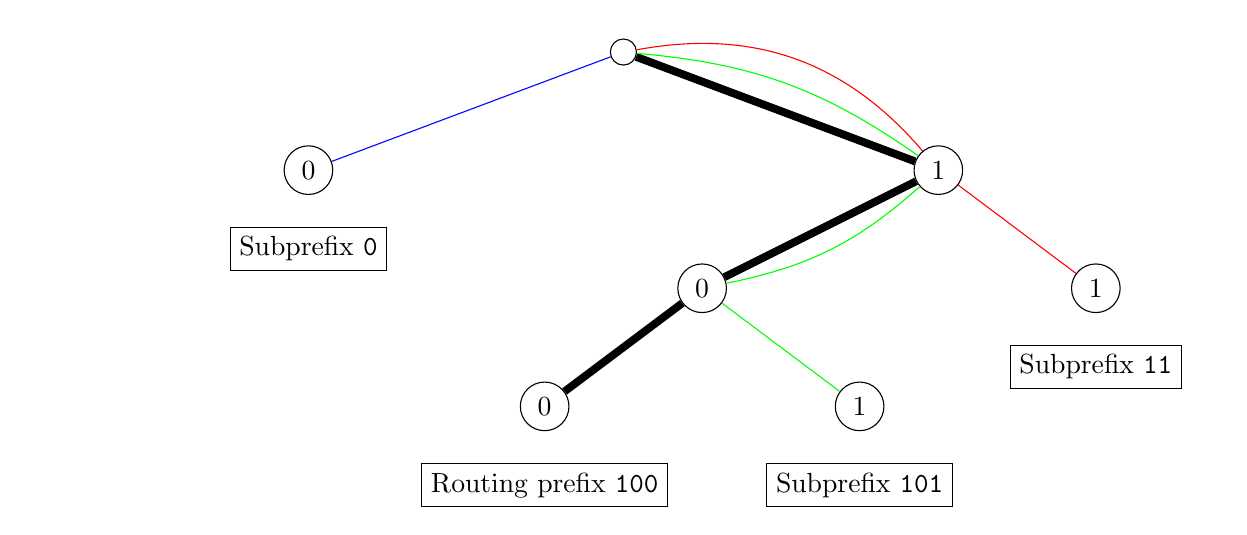
\begin{tikzpicture}
    \begin{scope}[every node/.style={circle, draw}]
      \node (0) at (0, 0) {};
      \node (10) at (-4, -1.5) {0};
      \node (11) at (4, -1.5) {1};
      \node[draw=none] (20) at (-6, -3) {};
      \node[draw=none] (21) at (-2, -3) {};
      \node (22) at (1, -3) {0};
      \node (23) at (6, -3) {1};
      \node[draw=none] (30) at (-7.4, -4.5) {};
      \node[draw=none] (31) at (-4.6, -4.5) {};
      \node[draw=none] (32) at (-3.4, -4.5) {};
      \node[draw=none] (33) at (-0.6, -4.5) {};
      \node (34) at (-1, -4.5) {0};
      \node (35) at (3, -4.5) {1};
      \node[draw=none] (36) at (4.6, -4.5) {};
      \node[draw=none] (37) at (7.4, -4.5) {};
    \end{scope}

    \begin{scope}[every node/.style={rectangle, draw, align=left}]
      \node (SP0) at (-4, -2.5) {Subprefix \texttt{0}};
      \node (SP11) at (6, -4) {Subprefix \texttt{11}};
      \node (RP100) at (-1, -5.5) {Routing prefix \texttt{100}};
      \node (SP101) at (3, -5.5) {Subprefix \texttt{101}};
    \end{scope}

    \draw[line width=1mm] (0) -- (11) -- (22) -- (34);
    \draw[color=blue] (0) -- (10);
    \draw[color=red] (0) edge[bend left] (11);
    \draw[color=red] (11) edge (23);
    \draw[color=green] (0) edge[bend left=15] (11);
    \draw[color=green] (11) edge[bend left=15] (22);
    \draw[color=green] (22) edge (35);

  \end{tikzpicture}
  \caption{Example of subprefixes illustrated on a tree. Edges to the left
  represent a \texttt{0}, edges to the right a \texttt{1}. The routing prefix of
  \texttt{100} is shown by thick black edges, the subprefixes \texttt{0},
  \texttt{11}, and \texttt{101} by colored ones.}
  \label{fig:subprefixes}
\end{figure}

\subsection{Reputation Management}
\label{sec:desc_rep_management}
Penalty delays can only be correctly applied if every peer in a query group is
aware of all of his query peer's reputations. To achieve this, every peer stores
all relevant reputations locally, and receives updates for them from query peers
in the same query group.

The reputation of a query peer is initialized to 0 upon his joining the group.
It is subsequently modified through \emph{reputation updates} shared in the
group. A reputation update can either contain a reward, increasing the
reputation of the peer whom it is regarding, or a penalty, decreasing it.

Rewards and penalties are awarded in response to an interaction with another
peer or peers. In case the two peers share more than one query group, they are
applied in all of those groups (letting the peer choose in which group he would
like to receive the reputation update is open to abuse: he could choose to
receive a penalty in a group he doesn't really care about).

Rewards and penalties are handled in different ways for incentive reasons
(Section~\ref{sec:desc_rationale} goes into more detail on peer incentives).
After a peer performs a cooperative action (one deserving a reward, e.g.
successfully responding to a query) on another peer, the other peer sends him a
\emph{cooperation confirmation}, which is a statement signed by the other peer
confirming that the peer performed the action. The peer then broadcasts this
statement to all peers in the query group, who then increase the reputation they
have stored for the peer by the amount the rules of the system dictate should be
awarded for the action.

After a peer performs a defecting action on another peer, it is the other peer
that broadcasts the message stating what the first peer did. The query peers
again update their reputation record. For penalties, the peer who was wronged
must broadcast the message, since the one about to receive a penalty clearly has
no incentive to do it himself. Strictly speaking, the other peer doesn't either,
since there is no immediate benefit for him doing so (peers are selfish, not
vengeful). So broadcasting the reputation update must also give the broadcaster
a (small) reward.

The reputations stored at the members of a query group of course can't be
perfectly synchronized due to network delays. So whenever a peer has to make a
decision that depends on another peer's or his own reputation, he must give some
leeway to account for this. He should accept any action of another peer's as
appropriate that is within the rules according to any of the reputation values
in the recent past.

Reputation updates must include a timestamp at which they should be applied in
order to correct for different arrival orders. Otherwise, the reputation record
may diverge at different peers if they receive 2 updates in a different order,
where one of them set the reputation to 0. Consider a peer with 1 reputation and
2 updates arrive: one subtracting 2, the next adding 1. Subtracting first yields
1 reputation, adding first yields 0. In case 2 updates specify the same time,
use the uint value of the ID of the peer who sent the update (this implies that
peers must not send two reputation updates with the same timestamp).

The complete reputation record must be made available to a new peer joining a
query group. It is simply copied from the \emph{entry peer}, the one who handles
the joining of the new member. But this opens up the possibility for a race
condition if the new peer joins right after a current member of the group sends
a reputation update. The new peer will not be sent the update, but the update
may not have arrived in time at the entry peer for him to give a current copy to
the new member.

To address this, every peer must include a sequence number with every reputation
update he sends within a query group. This number is incremented by 1 with every
update he sends. Every peer maintains the last sequence number received by every
peer in the group. When joining a query group, the new peer receives a copy of
the current group state from one of the peers, which includes the sequence
numbers. Then, after he is established in the group, the new peer can check with
another peer whether he is up to date by giving his current state of sequence
numbers, potentially receiving a correction. To incentivize another peer's
cooperation in this, a reward is applied, but only once per new peer.

\section{Rationale}
\label{sec:desc_rationale}
The goal of the system that was described is to exploit the peers' desire to use
the DHT in order to get them to contribute, thereby cultivating the wide variety
of peers to choose from. To achieve this, every action the system requires the
peers to do must have an incentive, i.e. not carrying out the action must carry
the threat of being less likely to use the system with a good quality of
service.

It should be considered, though, that just because an action is rewarded, there
is no guarantee that it will be carried out. If a peer considers his current
amount of reputation sufficient, he may opt to not carry out such an action. In
that case, the peer is said to be \emph{reputation saturated}.

This notion of a hard cutoff is actually a simplified view on a selfish peer's
motivation. In a more realistic setting, whether a peer carries out an action
that is rewarded depends on the magnitude of the reward and the cost of the
action, which he weighs against one another. Peers would only perform an action
iff the value of the added reputation exceeds the cost of performing the action.

In the simplification in the implementation, peers always aim to be cooperative
right until they reach their saturation reputation, which is determined by the
penalty threshold and the reputation buffer described in (see
Section~\ref{sec:impl_coop_defect_behavior}). This acts as a proxy for their
weighing cost of action agains value of reputation.

\subsection{The Reputation System}
\label{sec:desc_rep_system}
This is the purpose of the reputation system. Without reputation, peers only
receive a poor level of service in the form of artificial delays. Looking up
someone's reachability information is assumed to be done right before initiating
communication with the other party. Artificial delays in this situation would be
annoying to the user and are therefore a good incentive for peers to gain
reputation.

Rewards and penalties can then be used to incentivize desirable and
disincentivize undesirable behavior. Rewards are applied for properly responding
to a query, i.e. within the right time frame, and with the correct record.
Penalties are applied for not responding at all, responding too early or too
late, or not being able to resolve the target ID to the correct record.

Of course, late queries must be penalized in order to keep up the promise
of good service for high reputation. But, a little less intuitively, early
queries must also be penalized. Without any incentive to apply the correct
penalty delay, peers would be inclined to respond at the next convenient time.
In many cases, that might be right away, so that the peer doesn't have to keep
the state of the interaction stored for longer than necessary. Delaying the
response also requires the programmer of the implementation to do extra work.
The peer might conceivably also just respond whenever network resources are
free.

The problem with being indifferent to peers responding with no delay at all is
that it reduces or removes the threat of not participating. If there are
generous peers responding without delay independent of reputation, there is less
of no incentive to gain reputation. If the system's goal was availability alone,
this may be fine, but it is also supposed to offer peers a wide variety of peers
as query targets to choose from, so that profile building becomes more
challenging. Reducing the incentive to gain reputation, and thereby to respond
to queries, hinders this. The generous peers would attract a lot of queries and
have it easier to build profiles, counteracting one of the goals of the system.

\subsection{Query Groups}
Reputation gained by responding to one peer entitles a peer to better service
from other peers. This makes sense, since one of the goals of the system is to
allow peers to spread their queries to many peers. It has to be practical for
any pair of peers to have very few interactions but still use the reputation
system. Having every peer keep a local reputation for his communication partners
is therefore not an option, as many peers wouldn't be able to gain sufficient
reputation over these few interactions to be entitled to a reasonable quality of
service.

Tracking reputation globally doesn't scale to large networks. Peers can't
practically store every other peer's reputation locally and receive updates for
all of them. Moreover, spreading these updates throughout the network to so many
recipients would be challenging and require incentives. Storing reputation in a
decentralized structure like the DHT the system is supporting, or a wholly
separate one, would add additional delays. Before responding, each peer would
have to do a DHT lookup to even determine when to send the response. This would
have to happen at every hop in the query. Not to mention that this potentially
includes another DHT, the maintenance of which requires incentives itself.

The solution offered in this thesis are query groups, which are small enough
that each peer can store locally the reputations of the query peers, and updates
can be broadcast. At the same time, peers don't have to cultivate a trusting
relationship with a peer before they can query him, only with the query group as
a whole. Query groups become the unit in which peers build trust in each other's
willingness to cooperate.

This of course segments the network into many small groups, and the ideal goal
of being able to query any other peer is not reached. But peers wishing for more
privacy can join more query groups than is necessary to complete their subprefix
coverage, thereby increasing the pool of query peers. Of course, this comes at a
higher management cost.

Furthermore, query groups can be changed frequently, so that peers in them don't
become so familiar with one's querying habits that they can build a meaningful
profile. Before leaving an old group, it makes sense to join a replacement group
and gain reputation above the penalty threshold to ensure a smooth transition.
Doing so more frequently again adds cost at the benefit of higher privacy.

\subsection{Incentives for Repuation Management}
\label{sec:desc_incentives_rep_mgmt}
There must also be incentives for reputation updates. After receiving a
successful response to a query, the querying peer sends a cooperation
confirmation to the responder which entitles him to his reward. He then
broadcasts a reputation update benefitting himself. The incentive for this is
evident.

Broadcasting a penalty for another peer also has to give a small reward to the
one sending it, as otherwise there would be no incentive to do so. This is the
case even if the penalty is applied for defecting on the sender of the penalty,
like failing to respond in time, since we're only assuming peers are selfish,
not vengeful. They do not consider hurting someone who hurt them a benefit.

For this to work, however, the complaint system is crucial. If the querying peer
doesn't send the cooperation confirmation, and there is no recourse and no
threat of penalty for it, selfish peers will not do it. Similarly, it must not
be possible to apply penalties to other peers without cause, just for the
benefit of the reward broadcasting it brings.

The complaint system is sadly out of scope for this thesis, and likely to have
to deal with complex dynamics arising from the interaction of peers. If it
doesn't work, the entire system doesn't work.

Reputation should not be so plentiful that all peers in a query group can become
reputation saturated. If that should happen, no one has any incentive to respond
to queries, but no one has an incentive to broadcast penalties anymore, either.
Everyone would remain at their current, saturated reputation without any work
actually getting done. Section~\ref{sec:attenuation} describes how to adjust the
parameters of \emph{reputation attenuation} in order to control how often peers
become saturated.

A possible modification to defuse the situation should it happen anyway is to
let reputation decay at a slow rate. At a set interval, a fixed amount of
reputation is subtracted from each peer in every query group. This can be
implemented without actual reputation updates by viewing reputation relative to
the group's creation time: Every time a peer accesses a query peer's reputation,
he subtracts a fraction of the group's age from the value stored in the
reputation record. This requires reasonably well-synchronized clocks.
\emph{Reputation decay} was implemented in the simulation as the first approach
to keep peers interested in participating, but the threat of penalty for failing
to respond turned out to be enough.

Besides broadcasting reputation updates, peers receiving them also need to have
an incentive to update their local reputation record. After all, simply ignoring
an incoming message is easier than processing it. The incentive is indirect and
results from the fact that peers need to know the accurate reputation of their
query peers in order to apply the correct penalty delays and thus avoid
penalties.

\subsection{Incentives in Sync Groups}
\label{sec:desc_incentives_sync}
Incentives are also needed in sync groups, where peers stay up to date with the
records they're responsible for. Updates to records are broadcast by the owner
of the record (since every peer stores exactly one record under his own ID, sync
groups consist of the owners of the records the group is responsible for). The
to do so is simply that other peers can reach him.

But there also needs to be an incentive to even listen to and apply updates
within the sync group; it would be easier to just dismiss them and respond with
the old record when queried, or even claim that, no matter the target ID, no
record exists for it.

The incentive here is indirect: If a peer responds with an outdated record or
claims no record exists even though it does, the querying peer may apply a
penalty for an incorrect response if he notices. This is not guaranteed to
happen, since it requires the querying peer to send at least one redundant
query. It does not require the complaint system, though: The querying peer has
the (signed) response containing incorrect information, and a response from
another peer with the correct information (records themselves are signed by the
owner, so can't be forged), and can therefore prove the defecting behavior.

The penalty is not guaranteed to be applied for another reason: Even if the
querying peer sends a second query, the other responder may also give an
incorrect response. In the extreme case, all members of a sync group respond "no
such record" to every query and no one can ever receive a penalty for an
incorrect query. This would be an equilibrium for this particular part of the
system, but an unfortunate one, since none of the records of the peers in the
sync group ever make their way to an outside peer.

But if even one peer properly applies the updates, there is a threat of penalty:
There is a chance the querying peer sends a second query, and again a chance
that the response comes from one such peer. Then the querying peer will apply a
penalty. Depending on a peer's current reputation and the magnitude of the
penalty, this can seem like an acceptable risk. The penalty should therefore be
set sufficiently high to ensure that it does so rarely. If that is the case,
peers need to apply updates in order to even be able to respond correctly when
they are low on reputation. If they have the current information anyway when a
query arrives, the cost of responding correctly (looking up the record in
memory) shouldn't be much higher than just responding "no such record".

\subsection{Relative Amounts of Rewards and Penalties}
While not tested in experiment, some general rules for the relative proportion
of different rewards and penalties are apparent.

The penalty for letting a query time out should be greater than that for a fail
response (one which states the target ID couldn't be resolved). The latter is
more useful to the querying peer, since it takes less time and allows him to
e.g. send a retry sooner.

The reward for broadcasting a penalty should probably be less than any penalty,
otherwise it becomes easy for colluding peers to "penalize" each other, thus
gaining arbitrary reputation. Technically, the complaint system is supposed to
catch this, and there are considerations on how to limit collusion in
Section~\ref{sec:desc_collusion_sybil_attacks}, but it seems ill-advised to make
this kind of behavior possible in the first place.

The penalty for an incorrect response should be set sufficiently high to
disincentivize them even if the likelihood of actually receiving the penalty is
low (see Section~\ref{sec:desc_incentives_sync}).

\subsection{The Recursive Query Problem}
\label{sec:desc_rec_query_prob}
Recursive queries can lead to the \emph{recursive query problem}, which is a
peer's bad reputation in one query group having adverse effects on his
reputation in another. It is illustrated in
figure~\ref{fig:recursive_query_problem}. Say peer A receives a query from peer
B, and they share query group 1. A needs to send the query on to one of his
query peers in order to answer it, and determines that peer C is the most
suitable recipient, whom he knows from query group 2. A is expected to respond
to B within a time window determined by B's reputation in group 1. Similarly, C
is expected to respond to A within a time window determined by A's reputation in
group 2. If minimum delay of the latter time window is greater than the maximum
delay of the former, A has no chance of responding in time (that is assuming C
observes the expected delay) and will be penalized for it.

\begin{figure}[t]
  \centering
  \begin{tikzpicture}
    \begin{scope}[every node/.style={circle, draw}]
      \node (A) at (-3cm, 0) {A};
      \node (B)[align=left] at (0, 0) {B};
      \node (C) at (3cm, 0) {C};
      \node[draw=none, align=justify] (reps) at (-7cm, 0) {
        \textbf{Reputation}\\
        \begin{tabular}{|l|c|c|}
        \hline
        \rowcolor{slightgray}
        \T & group 1 & group 2\B\\
        \hline
        \cellcolor{slightgray}\T A & 10 & -\B\\
        \hline
        \cellcolor{slightgray}\T B & 10 & 6\B\\
        \hline
        \cellcolor{slightgray}\T C & - & 10\B\\
        \hline
        \end{tabular}
      };
    \end{scope}

    \begin{scope}[every node/.style={midway}]
      \path (A) edge[->, thick, above, bend left=30] node[xshift=-0.4cm]
        {\textbf{1:} query at 0} (B);
      \path (B) edge[->, thick, above, bend left=30] node[xshift=0.4cm]
        {\textbf{2:} query at 0.1} (C);
      \path (C) edge[->, thick, below, bend left=30] node[xshift=0.4cm]
        {\textbf{3:} response at 4.1} (B);
      \path (B) edge[->, thick, below, bend left=30] node[xshift=-0.4cm]
        {\textbf{4:} response at 4.2} (A);
    \end{scope}

    \begin{pgfonlayer}{background}
      \begin{scope}[every node/.style={
        circle,
        inner sep=0,
        inner xsep=0.3cm,
        inner ysep=0pt,
        opacity=0.5
      }]
        \node[fit=(A)(B), fill=red!30, rotate=0,
              label={[label distance=-1cm]90:query group 1}] {};
        \node[fit=(B)(C), fill=violet!30, rotate=0,
              label={[label distance=-1cm]90:query group 2}] {};
      \end{scope}
    \end{pgfonlayer}
  \end{tikzpicture}
  \caption{Illustration of the recursive query problem. The penalty threshold is
  10. Peer B receives a query from peer A and is expected to respond without
  imposing a penalty delay. He has to query peer C, but only has 6 reputation in
  the query group he shares with him. C imposes a 4-second penalty delay, so B
  can't respond to A's query in time and will incur a penalty.}
  \label{fig:recursive_query_problem}
\end{figure}

Under these circumstances, A's bad reputation in group 2 leads to a penalty in
group 1. This is potentially a serious hindrance to a peer's ability to gain
reputation. Under unfortunate circumstances, one could imagine low reputation
values in two query groups keeping each other down. This problem can also be
observed in the simulation results, see
Section~\ref{sec:rep_avail_rec_query_prob}.

While the recursive query problem can impede peers' ability to gain reputation,
there is an argument that it can be a good thing once peers have sufficient
reputation. It forces them to maintain good subprefix coverage with a good
quality of service, even if they may not care about parts of the ID namespace
personally.

\subsection{Empty Sync Groups}
\label{sec:desc_empty_sync_groups}
There may be a routing prefix for which there is no peer, i.e. the corresponding
sync group is empty. In that case, there is no one who can authoritatively
answer queries for this prefix (stating that no peer exists). Such queries are
still legitimate, e.g. because there used to be a peer with the routing prefix
in question. But more importantly, they occur when the empty routing prefix is
the subprefix of some peer. That peer will send a prefix query to complete his
subprefix coverage but never receive an authoritative response. Peers close to
the empty sync group (sync peers of the peer, whose routing prefix is equal to
the empty one except in the final bit) could respond that there probably doesn't
exist a peer, but this isn't ideal.

The only workaround that can be offered is to choose the routing prefix length
in such a way that empty sync groups don't occur. It must be variable during
operation anyway, in order to support changes in network size. This can be
achieved e.g. through a system like the one described in
Section~\ref{sec:desc_load_balancing}, but maybe also a simpler one, in which
the routing prefix length is the same for all peers, but can be changed at
runtime.

Besides empty sync groups, groups with only very few peers cause problems as
well, as they make peers' ability to gain reputation brittle, as described in
Section~\ref{sec:rep_avail_small_sync_groups}.

\subsection{Circular Queries}
There is nothing in the system in principle that prevents peers from querying a
peer who is not closer to the target ID than they are themselves. If they do,
circular queries, or routing loops, can occur, in which peer A queries peer B,
who queries peer C, who queries peer A again. Without any way of detecting such
loops, peer A may even think that he can use the response to his initial query
to answer the query he received from C, and not query anyone else. Then all
queries will time out and everyone (including peer A) receive a penalty, even if
all involved were trying to cooperate.

There are no incentives specifically in place to get peers to only query peers
closer to the target ID. Usually of course, it is better for a peer to query the
closest peer since that reduces the number of hops required and thus the
response time. But if the peer has low reputation in all the query groups he
shares with peers closer to the target ID, it is the rational choice to instead
query one who is not closer from a group in which he has high reputation. The
absence of the penalty delay is likely to make up for the additional hops.

Forbidding such queries entirely isn't an option either, since they are
sometimes necessary. In particular for new peers looking to complete their
subprefix coverage. They have to query peers not closer to the subprefix they're
querying for, since they don't know anyone closer (that's why they're doing it,
after all). It might be an option to respond to such queries, but give a large
penalty for posing them. That wouldn't affect new peers, who have no reputation
yet anyway, while disincentivizing the behavior for established peers.

\chapter{Implementation}
\label{chap:implementation}
A simulation has been implemented using the SimPy discrete event simulation
framework\footnote{The software is available on github.com at
\url{https://github.com/dddsnn/name-lookup-incentives}.}. It simulates a network
of selfish peers providing and accessing a DHT implementing the system described
in the previous chapter.

Parameters of the simulation are set via a \texttt{.settings} file, which is
supposed to make results of simulation runs reproducible\footnote{The simulation
uses floating-point arithmetic, which is a possible source of indeterminism
between different systems\cite{dawson2013determinism}. On the same system,
results should be reproducible.}. Parameters for the default settings, along
with some explanation, can be found in Section~\ref{sec:app_default_settings}.
They are chosen in such a way that the dimensionless time units of the
framework can be viewed as seconds.

\section{Initialization}
Before the simulation starts, the environment is initialized. This involves
generating IDs for all the peers, creating the peer objects, and introducing
each peer to a few others.

The IDs are generated randomly, although there are some options that can
influence this by forcing all sync groups to be non-empty, or even have the same
sizes (sync groups are determined by the routing prefix, which is a part of the
ID).

Once all peers are created, they are introduced to other peers, i.e. given their
ID and network address such that they can communicate with them. Each peer is
introduced to all of his sync peers as well as a number of randomly selected
peers with which he may from query groups (the random sample may also contain
sync peers and himself). Afterwards, every peer's process to complete the
subprefix coverage is queued up to run once the simulation starts.

Finally, another process is started that facilitates traffic. Every second, one
request for a full ID is generated at every peer. A request represents a user
interacting with the protocol stack. It may lead to the peer needing to send out
a query in order to resolve it, but it may not (if the peer already knows the
answer, e.g. if the requested ID is in the same sync group). The requested ID is
randomly chosen with equal distribution from all existing peer IDs and may be
the peer's own ID.

\section{Peer Behavior Model}
\subsection{Completing Subprefix Coverage}
Peers are introduced to a number of other peers once during initialization, but
every time they receive a successful response they are introduced to the peer
whose information is contained in the response.

When a peer is introduced to another one he doesn't already know, he checks
which of his subprefixes the other peer serves. If he already knows enough peers
serving that subprefix, he doesn't do anything. Otherwise, he will join a query
group with the new peer.

This process of joining a query group is simplified: All peers have access to a
list of all query groups. The peer will first check if there is a query group
the other peer is in that is not full. If so, he will add himself to that group.
Otherwise, he will check if any of his own query groups is not full and, if so,
add the other peer to it. Otherwise, he will create a new query group containing
just himself and the other peer. A query group is considered full once its size
reaches a number adjustable in the settings, which is the same for all peers.
There is no further mechanism to prevent query groups from becoming too big.

Each peer repeatedly, after a fixed interval, runs a process that attempts to
complete the peer's subprefix coverage. The peer for which of his subprefixes he
knows fewer peers than he'd like and sends queries for these subprefixes. Once a
successful response arrives, the peer information contained in it is introduced
and a query group can be joined. In those queries, the peer specifies which
peers covering the subprefix he already knows, so they will not occur in the
response. The queries are also special in that peers can select recipients that
are further away from the target ID. This is usually disallowed to prevent
routing loops. However, when completing subprefix coverage, they may be
necessary: if the peer doesn't know anyone closer to the desired subprefix (and
that is the problem he is trying to solve), he must necessarily query someone
who is not closer. There is no mechanism to prevent routing loops implemented.

\section{Cooperative/Defecting Behavior}
\label{sec:impl_coop_defect_behavior}
Peers are modeled to be selfish with regards to their willingness to cooperate.
They behave cooperatively and do their best to respond to incoming queries
within the correct time window while they are not yet reputation saturated.
They are saturated once their reputation in the relevant query group (the one
shared with the peer sending a query) is at least the penalty threshold
reputation plus the \emph{reputation buffer}. If they share more than one query
group with the querying peer, they consider their minimum reputation, since they
will receive rewards and penalties in all those groups.

If they receive a query and are reputation saturated, they will ignore it
(eventually causing a timeout at the sender), but expect to receive a penalty
for doing this. That means they store an expectation in all the relevant query
groups that their reputation there will be reduced by a penalty in the future.
Once the penalty is actually applied, they delete the record of the expectation.
When determining whether they are reputation saturated, they take into account
the expectations they have stored. In effect, once they ignore a query, they
expect a penalty and thus are immediately not saturated anymore.

The reputation buffer is a configurable parameter determining how long peers
stay cooperative before they defect for the first time. It is a simplification
that acts as a proxy both for the peers' valuation of reputation, as well as the
cost of cooperating. Essentially, peers give reputation infinitely high value
while they have less than the saturation reputation, and no value otherwise.
This makes it impossible for them to factor the cost of the action requested of
them into their decision.

When peers are trying to resolve a target ID, they only send one query at a
time. Only once that query has failed do they send a query to the next viable
peer. For each target ID they are trying to resolve, they note which peers they
have already queried and don't try them again. If all viable peers have been
tried, they consider the query to have failed.

No complaint system has been implemented, so simplified reputation updates are
used: Peers simply broadcast reputation updates faithfully and honestly, not
considering any incentive for doing so. When a response arrives or a timeout
occurs, they send an update to each member in all the query groups they share
with the responder. Contrary to the system description, even for successful
responses it is the peer who sent the query that broadcasts the reputation
update, not the one who responded successfully.

\section{Simplifications}
The implementation contains a number of simplifications compared to the system
described in Chapter~\ref{chap:system_description}.

\begin{itemize}
\item As already mentioned, there is no complaint system. Any actions that may
require it, like reputation updates, are always executed faithfully.

\item Query group creation and joining is simplified in that peers can simply
add themselves to any query group they like, and even add other peers to an
existing query group without that peer having any say in this. For this purpose,
peers have access to a complete list of all existing query groups that is shared
among all peers. Creating a new query group is done by placing a new object in
that list.

\item There is no way for peers to join query groups other than through the
mechanism to complete their subprefix coverage. There is also no way at all to
leave a query group. This leads to some very small groups, usually a few with
just two peers. In these groups, reputation gains are very slow because of the
low amount of traffic.

\item Peers never go offline, change their addresses or update the record they
store in the DHT.

\item Peers respond to all queries, even from peers they don't share a query
group with. For those, they apply the maximum penalty delay.

\item Peers never respond too early, and hence there is no mechanism implemented
to penalize this.

\item Peers don't give any leeway when checking another peer's reputation. When
deciding the penalty delay, the current reputation is used, even if e.g. the
sender of the query had more reputation when he sent it and is thus expecting a
faster response.

\item No encryption or signing of messages is actually taking place.
\end{itemize}

\section{Analysis Module}
When the simulation is running, a log is kept of all interesting events like
queries or responses being sent or timing out. Once the simulation is done, this
log is written to a file that allows to examine the behavior of the system.

The \texttt{analyze} module is capable of creating various plots concerning the
system behavior.
\begin{description}
\item[Reputation percentiles] Illustrates the development of reputation of the
members of one query group over time. The reputation of the 5th, 25th, 50th,
75th and 95th percentile of reputation is plotted with one graph each. Note that
in many cases, query groups have 16 members, and so the 5th and the 95th
percentile represent only one peer. The penalty threshold reputation as well as
the saturation reputation are indicated by horizontal lines.
\item[Peer reputations] Illustrates the reputation values of one peer in all of
the query groups he is in over time. The reputation for each group is shown as a
separate graph. Optionally, a bar graph in the background shows the fraction of
the peer's responses that suffers from the recursive query problem (i.e. the
peer tried to respond, but once he was able, it was too late already). This plot
also includes horizontal lines indicating the penalty threshold reputation and
the saturation reputation.
\item[Response statuses] Illustrates the status of responses within the
simulation over time. The statuses \emph{success}, \emph{failure} and
\emph{timeout} should be self-explanatory. A response can be \emph{unmatched} if
peer A sends a query to peer B, the query then times out at A, but B responds
(late) anyway. By that time, A has deleted the record of having sent a query to
B and thus can't match the response to an outgoing query. This frequently occurs
with the recursive query problem. The status \emph{returned\_excluded\_peer}
denotes the situation where a query was sent where certain IDs were excluded,
i.e.  unwanted as a response, but returned in the response anyway. This doesn't
happen in the simulation.
\end{description}

\chapter{Reputation Availability}
- peers who are behaving well must be able to attain and maintain enough
  reputation for delay-free service

\section{TODO}

\chapter{Selfish Peers}
\section{TODO}

\chapter{Performance}
\label{chap:performance}
- define messages, estimate sizes, id lengths etc.
    - remember signatures for size
    - remember public key for size of a record (or use a separate record to map
      key fingerprint to full key?)
    - remember last changed time (to determine if a received record is very old
      and to give a penalty in that case)
    - remember (possibly?) ttl
    - reputation update regarding responses have to state which ID the query was
      for if peer selection overlap-rep-sorted is used, so that the lowest-rep
      peer can detect that he should have been sent a query
- reputation updates could potentially be batched to save overhead
- compare with tit-for-tat
\section{Performance Indices}
TODO
\section{Comparison with Plain DNS}
\section{Comparison with Tor}
- tor fully anonymizes tcp, stronger than what we do here
    - specify hostname when establishing a connection, exit nodes does dns
      lookup
    - Remote hostname lookup is basically dns over the circuit, (but only A and
      AAAA records)
- latency is what's important to us, ignore tor's establishing a circuit and our
  finding query groups, that can be done in the background
- queries not optimizable for geography, worst case every hop towards the other
  end of the planet
- ignore possible tcp delay from dropped packets, hol blocking, assume network
  not congested?
\subsection{Tor}
- fixed-size cells of 512 bytes
- assuming link protocol version 4
- remote hostname lookup: 512 bytes fixed-length cell, query and response each
- or let the exit node do the lookup and include the first payload. with a small
  http request, lookup is basically free, same as a dns query
- but tor has no incentives (cite tor perf improvements paper)
TODO

\chapter{Conclusion}
\label{chap:conclusion}
This thesis proposed a reputation system for a DHT storing reachability
information that is meant to increase participation so that queries can be
spread out among many recipients.

Broadly speaking, there are three elements of the system that are absolutely
integral and need to be investigated. They are firstly the availibility of
reputation to cooperative peers, which is necessary to make the system useful to
them. Secondly, a way of creating, joining and leaving query groups that allows
peers to effectively find others that they need to forward their queries. And
lastly, the complaint system, which is necessary to prevent abuse of the
reputation system.

The first of these has been examined in this thesis via simulation. With the
implementation as it is, the results are encouraging so far. They show, with
some caveats, that selfish peers are able to gain enough reputation to be
entitled to delay-free service, under the assumption that they can be motivated
to contribute by the promise of a good quality of service.

The other two have not been implemented, but some ideas presented. If those are
implemented, they are likely to influence each other, as well as the reputation
availability in ways that are difficult to predict. It may well turn out that
the ideas presented in this thesis can not be completed into an effective
system.

With regards to latency, the system compares very unfavorably to DNS, likely
being several times slower. This is not surprising, given that their purposes
are not precisely the same. The purpose of DNS is to provide resolutions from
authoritative servers quickly, whereas the DHT is focused on robustness and
reliability. Queries in the DHT are also not optimized for proximity between
peers.

Some possible attacks on the system, ones exploiting the reputation system, as
well as ones seeking to circumvent the privacy gains, have been described and
possible countermeasures discussed.


%%%%%%%%%%%%%%%%%%%%%%%%%%%%%%%%%%%%%%%%%%%%%%%%%%%%%%%%%%%%%
%% LITERATUR UND ANDERE VERZEICHNISSE
%%%%%%%%%%%%%%%%%%%%%%%%%%%%%%%%%%%%%%%%%%%%%%%%%%%%%%%%%%%%%
%% Ein kleiner Abstand zu den Kapiteln im Inhaltsverzeichnis (toc)
\ifnotdraft{
\addtocontents{toc}{\protect\vspace*{\baselineskip}}
\cleardoublepage
%% Literaturverzeichnis
\phantomsection % phantomsection wird benötigt, damit z.B. hyperref die richtige Seite verlinkt.
\addcontentsline{toc}{chapter}{Bibliography}
%\nocite{*} %Auch nicht-zitierte BibTeX-Einträge werden angezeigt.
\bibliography{literature/literature}%Eine Datei 'literatur.bib' wird hierfür benötigt.
\bibliographystyle{styles/acmurl}%Art der Ausgabe: plain / apalike / amsalpha / ...
}

%% Abbildungsverzeichnis
%\clearpage
%\addcontentsline{toc}{chapter}{List of Figures}
%\listoffigures

%% Tabellenverzeichnis
%\clearpage
%\addcontentsline{toc}{chapter}{List of Tables}
%\listoftables


%%%%%%%%%%%%%%%%%%%%%%%%%%%%%%%%%%%%%%%%%%%%%%%%%%%%%%%%%%%%%
%% ANHÄNGE
%%%%%%%%%%%%%%%%%%%%%%%%%%%%%%%%%%%%%%%%%%%%%%%%%%%%%%%%%%%%%
\appendix
\chapter{Appendix}
\section{Definitions}
\begin{description}
\item[Record:] The data stored in a DHT under one key (or \emph{record ID}).
Also contains a timestamp giving the time of last change.
\item[Peer:] One participant of the system, has one unique \emph{ID}; commonly
called \emph{node} in the context of DHT.
\item[ID, Peer ID:] A bit string the length of which is fixed and prescribed by
the \emph{rules of the system}. Uniquely identifies a peer.
\item[Record ID:] A bit string of the same length as a \emph{peer ID}. Uniquely
identifies the record belonging to the peer with the same ID. Technically the
key of the record, but the word ID is used to stress that it's of the same kind
as a peer ID.
\item[Reachability information:] The abstract notion of information stored in
records in the DHT that is sufficient to communicate with a peer. More
concretely, an IP address.
\item[Target ID:] A bit string that is the subject of a \emph{query}. Its length
is less than or equal to that of a \emph{peer ID}. If less, the query is asking
for any peer whose ID starts with the target ID.
\item[Matching an ID:] Two ID's match iff one is a prefix of the other. E.g., a
\emph{target ID} matches a \emph{peer ID} (or a \emph{record ID}) if the target
ID is a prefix of the peer ID, i.e., the peer ID is a valid response for a query
asking for the target ID.
\item[Overlap $o(a, b)$:] The length of the longest common prefix of two bit
strings. Defined in Section~\ref{sec:desc_querying}.
\item[Being closer to an ID:] ID A is closer to ID X than ID B iff the overlap
of A and X is greater than that of B and X.
\item[Routing prefix:] The prefix of a \emph{peer ID} of a length that is equal
for all peers and prescribed by the \emph{rules of the system}. Determines which
\emph{sync group} a peer is in.
\item[Being responsible for a routing prefix:] A peer is responsible for a
routing prefix iff the routing prefix is a prefix of his ID, i.e. he is in the
\emph{sync group} associated with that routing prefix.
\item[Sync group:] A group of peers who are \emph{responsible for} the same
routing prefix. Maintain contact in order to exchange updates regarding the
records they store.
\item[Sync peer:] Peers A and B are sync peers of one another iff they are in
the same \emph{sync group}.
\item[Authority (with regards to a sync group/peer):] Sync groups or peers are
an authority, or authoritative, for their routing prefix because they are
responsible for keeping current with updates to its records.
\item[Query group:] A group of peers that may send each other \emph{queries}.
Maintain contact in order to track each other's reputation within the group.
\item[Query peer:] Peers A and B are query peers iff they are in the same
\emph{query group}.
\item[Subprefix:] A prefix of a \emph{routing prefix} where
the last bit is flipped. Each peer has a number of subprefixes equal to the
length of the routing prefix.
\item[Serving a subprefix:] Peer A serves subprefix P for peer B iff P is a
subprefix of B's and a prefix of A's routing prefix.
\item[Subprefix coverage:] The state of a peer's ability to forward queries,
which is dependent on having query peers serving subprefixes. The subprefix
coverage is complete iff, for each of his subprefixes, the peer has a query peer
serving it.
\item[Request (for a target ID):] External stimulus to the system prompting it
to resolve the target ID. Simulates interaction of e.g. a user with the protocol
stack. Not to be confused with a \emph{query}.
\item[Query (for a target ID):] Message sent from one peer (the querying peer)
to another (the recipient) requesting the \emph{record} for the target ID.
\item[Response, fail response:] Message sent from one peer (the responding peer)
to another to answer a \emph{query}. The responder may claim to have included
the correct record, making the response successful, or that he is unable to
resolve the correct record, making it a fail response.
\item[Usefulness:] A measure of how useful or important peer B is to peer A to
complete subprefix coverage. Based on the length of subprefix B can serve for A,
but can also incorporate the trust in A or how many other peers A knows also
serving that subprefix. Used by B to estimate how many queries he is likely to
get from A, or from an entire group of peers (see
Section~\ref{sec:desc_usefulness}).
\item[Reputation:] A non-negative, real number stored in every query group for
each of its members. Earned by peers for better quality of service.
\item[Reputation record:] The copy of all of a peer's query peers' reputation
stored locally.
\item[Reputation decay:] Process that subtracts reputation from every peer in a
query group at a steady rate.
\item[Reward, penalty:] A change in a peer's reputation respectively increasing
or decreasing it.
\item[Cooperative action:] An action performed by a peer that warrants a reward.
\item[Defecting action:] An action performed by a peer that warrants a penalty.
\item[Tremble:] A defecting action that was not intended by the peer, but e.g.
caused by a congested network.
\item[Cooperation confirmation:] A signed statement given to another peer
confirming that he performed a cooperative action.
\item[Reputation attenuation:] A reduction of the magnitude of rewards that
takes effect once a peer's reputation passes a minimum (see
Section~\ref{sec:attenuation}).
\item[Raw and effective reputation:] Reputation before and after
\emph{reputation attenuation} takes effect.
\item[Recursive query:] A query in which the recipient performs all further
querying on behalf of the sender and returns the final result.
\item[Iterative query:] A query in which the recipient only indicates the next
suitable peer to query, the sender must perform the query himself. Requires
\emph{query vouchers} to provide a good level of service (see
Section~\ref{sec:desc_recursive_vs_iterative}).
\item[Query voucher:] A one-time-use statement entitling one peer to the level
of service of another. Used for iterative queries.
\item[Routing loop:] Failure in looking up a record in the DHT caused by at
least one peer in the chain of queries forwarding the query to a peer who is not
\emph{closer to} the \emph{target ID}. The query is sent back to peers who
originally sent it. See also Section~\ref{sec:selection}.
\item[Entry peer:] A peer who is a member of a query group and facilitates the
joining of another peer into that group.
\item[Recursive query problem:] An issue in which a peer's low reputation in one
query group negatively affects his reputation in another (see
Section~\ref{sec:desc_rec_query_prob}).
\item[Penalty delay:] The delay that is deliberately imposed before responding
to a query to penalize the querying peer.
\item[Penalty threshold reputation (short: penalty threshold):] The minimum
reputation a peer must have in order for the penalty delay to be 0.
\item[Saturation reputation, being saturated:] The amount of reputation at which
a peer considers himself to have enough and isn't motivated to do work in order
to earn more.
\item[Broadcast:] The spreading of the same message to all peers in some group.
Explicitly \textbf{not} necessarily an actual broadcast on the network layer,
may also be executed as multiple unicasts. The term is used for simplicity of
discussion.
\end{description}

\section{Default Settings}
\label{sec:app_default_settings}
Table~\ref{tab:default_settings} lists the values for a selection of the most
important parameters in the default settings. Below, some of the ones that
aren't quite self-explanatory are explained more closely. All possible
parameters are available in the code repository in the commented default
settings file \texttt{simulation/default.settings}, relative to the repository
root (TODO check).

\begin{longtable}{|l|l|}
\hline
\rowcolor{slightgray} \T Key & Value \B\\
\hline
\cellcolor{slightgray}\T \texttt{rng\_seed} & 5803379951609632196 \B\\
\hline
\cellcolor{slightgray}\T \texttt{peer\_batches} & \texttt{[(0, 64, \{\})]} \B\\
\hline
\cellcolor{slightgray}\T \texttt{num\_random\_introductions} & 8 \B\\
\hline
\cellcolor{slightgray}\T \texttt{even\_sync\_groups} & \texttt{False} \B\\
\hline
\cellcolor{slightgray}\T \texttt{initial\_reputation} & 0 \B\\
\hline
\cellcolor{slightgray}\T \texttt{force\_one\_group} & \texttt{False} \B\\
\hline
\cellcolor{slightgray}\T \texttt{ensure\_non\_empty\_sync\_groups} & \texttt{True} \B\\
\hline
\cellcolor{slightgray}\T \texttt{id\_length} & 16 \B\\
\hline
\cellcolor{slightgray}\T \texttt{prefix\_length} & 4 \B\\
\hline
\cellcolor{slightgray}\T \texttt{ignore\_non\_existent\_subprefixes} & \texttt{False} \B\\
\hline
\cellcolor{slightgray}\T \texttt{transmission\_delay} & 0.1 \B\\
\hline
\cellcolor{slightgray}\T \texttt{successful\_query\_reward} & 1 \B\\
\hline
\cellcolor{slightgray}\T \texttt{failed\_query\_penalty} & -1 \B\\
\hline
\cellcolor{slightgray}\T \texttt{timeout\_query\_penalty} & -2 \B\\
\hline
\cellcolor{slightgray}\T \texttt{no\_penalty\_reputation} & 10 \B\\
\hline
\cellcolor{slightgray}\T \texttt{reward\_attenuation $\rightarrow$ type} & \texttt{exponential} \B\\
\hline
\cellcolor{slightgray}\T \texttt{reward\_attenuation $\rightarrow$ exponent} & 0.35 \B\\
\hline
\cellcolor{slightgray}\T \texttt{reward\_attenuation $\rightarrow$ coefficient} & 1 \B\\
\hline
\cellcolor{slightgray}\T \texttt{reward\_attenuation $\rightarrow$ lower\_bound} & 10 \B\\
\hline
\cellcolor{slightgray}\T \texttt{reward\_attenuation $\rightarrow$ upper\_bound} & 15 \B\\
\hline
\cellcolor{slightgray}\T \texttt{reputation\_buffer} & 4 \B\\
\hline
\cellcolor{slightgray}\T \texttt{query\_peer\_selection} & \texttt{overlap\_rep\_sorted} \B\\
\hline
\cellcolor{slightgray}\T \texttt{query\_sync\_for\_subprefixes} & \texttt{False} \B\\
\hline
\cellcolor{slightgray}\T \texttt{uncovered\_subprefix\_interval} & 10 \B\\
\hline
\cellcolor{slightgray}\T \texttt{min\_desired\_query\_peers} & 2 \B\\
\hline
\cellcolor{slightgray}\T \texttt{max\_desired\_group\_size} & 16 \B\\
\hline
\cellcolor{slightgray}\T \texttt{query\_timeout} & 2 \B\\
\hline
\cellcolor{slightgray}\T \texttt{expect\_penalties} & \texttt{True} \B\\
\hline
\cellcolor{slightgray}\T \texttt{tremble\_chance} & 0 \B\\
\hline
\caption{Default values of a selection of settings.}
\label{tab:default_settings}
\end{longtable}

\begin{description}
\item[\texttt{peer\_batches}] A list of tuples \texttt{(time, number\_of\_peers,
settings)} that allows to add peers at different times and with individual
settings.
\item[\texttt{num\_random\_introductions}] Upon initialization, each peer is
introduced to a random sample of peers. This is the size of that sample.
\item[\texttt{even\_sync\_groups}] If \texttt{True}, initialization will take
care to make all sync groups the same size. This can be helpful in ruling out
unevenly sized sync groups as the cause of some observed effect.
\item[\texttt{force\_one\_group}] If \texttt{True}, all peers will be forced
into one query group. Can be helpful e.g. to rule out the recursive query
problem as the cause of some effect.
\item[\texttt{ensure\_non\_empty\_sync\_groups}] If \texttt{True},
initialization takes care that each sync group contains at least one peer.
\item[\texttt{prefix\_length}] Length of the routing prefix, which is just
called prefix in the simulation.
\item[\texttt{ignore\_non\_existent\_subprefixes}] If \texttt{True}, peers make
use of global information they are given in the beginning in order to not query
for subprefixes for which there doesn't exist a peer (i.e. the sync group is
empty) when they are completing their subprefix coverage. This is useful in
preventing ongoing querying for IDs that will never lead to a successful
response.
\item[\texttt{no\_penalty\_reputation}] The penalty threshold reputation.
\item[\texttt{reputation\_buffer}] The amount of reputation above the penalty
threshold peers need to have in order to consider themselves reputation
saturated.
\item[\texttt{query\_sync\_for\_subprefixes}] If \texttt{True}, peers will also
send queries to their sync peers (even if they are not query peers) when they
are completing their subprefix coverage.
\item[\texttt{uncovered\_subprefix\_interval}] Peers repeatedly check whether
they have complete subprefix coverage and send queries in order to complete it
if they don't. This is the time interval between checking.
\item[\texttt{expect\_penalties}] If \texttt{True}, peers expect to be penalized
when they perform a defecting action.
\item[\texttt{tremble\_chance}] The chance that a peer fails to respond to a
query, no matter whether he actually wanted to. Used to simulate the impact of
network failures etc.
\end{description}


\begin{figure}[t]
\centering
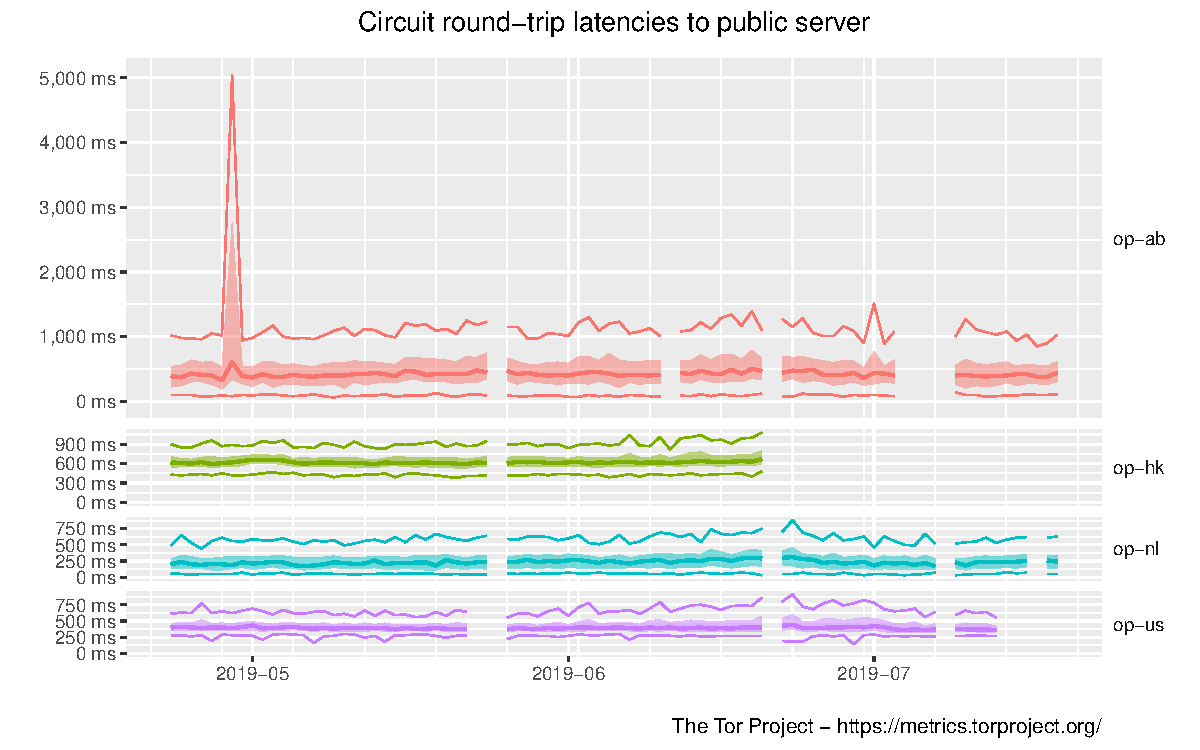
\includegraphics[width=1\columnwidth]{figures/onionperf-latencies-public-2019-04-23-2019-07-22}
\caption{Tor circuit RTTs from the Tor Project's metric site\cite{torperf}}
\label{fig:tor_rtt}
\end{figure}


\end{document}
